\documentclass[9pt,twocolumn,twoside,lineno]{main_class_file}
% Use the lineno option to display guide line numbers if required.


\usepackage[flushleft]{threeparttable}	% Allows for three part tables with a specified notes section
\usepackage{graphics}
\usepackage{amsmath}

\usepackage{tabularx}


\templatetype{main_style_file} % Choose template
% {pnasresearcharticle} = Template for a two-column research article
% {pnasmathematics} %= Template for a one-column mathematics article
% {pnasinvited} %= Template for a PNAS invited submission

\title{Polite speech emerges from competing social goals}

% Use letters for affiliations, numbers to show equal authorship (if applicable) and to indicate the corresponding author
\author[a,1,2]{Erica J. Yoon}
\author[a,1]{ Michael Henry Tessler}
\author[a]{Noah D. Goodman}
\author[a]{Michael C. Frank}

\affil[a]{Department of Psychology, Stanford University}

%\author{Erica J. Yoon\textsuperscript{1, *, †}, Michael Henry Tessler\textsuperscript{1, †}, Noah D. Goodman\textsuperscript{1}, \& Michael C. Frank\textsuperscript{1}}
%\affil{
%\vspace{0.5cm}
%      \textsuperscript{1} Department of Psychology, Stanford University\\
%      \textsuperscript{*} Corresponding author\\
%      \textsuperscript{†} These authors contributed equally to this work.  }

% Please give the surname of the lead author for the running footer
\leadauthor{Yoon, Tessler}

% Please add here a significance statement to explain the relevance of your work
\significancestatement{Standard views of language use emphasize its role in information transfer. On these views, the ubiquity of politeness is a puzzle. We present a new quantitative viewpoint on social language use that resolves the puzzle by assuming that speakers balance three potentially conflicting goals: an informational goal (\emph{be informative}), a social goal (\emph{be nice}), and a self-presentational goal (\emph{look nice}). This formal work provides a framework for developing a quantitative understanding of social language use more broadly. Further, by providing a theory of how speakers consider the feelings of others in formulating their utterances, it paves the way for the development of courteous computational agents.}

% Please include corresponding author, author contribution and author declaration information
\authorcontributions{Please provide details of author contributions here.}
\authordeclaration{Please declare any conflict of interest here.}
\equalauthors{\textsuperscript{1}E.J.Y. and M.H.T. contributed equally to this work.}
\correspondingauthor{\textsuperscript{2}To whom correspondence should be addressed. E-mail: ejyoon@stanford.edu}

% Keywords are not mandatory, but authors are strongly encouraged to provide them. If provided, please include two to five keywords, separated by the pipe symbol, e.g:
  \keywords{politeness $|$ computational modeling $|$ communicative goals$|$ pragmatics}

\begin{abstract}
Language is a remarkably efficient tool for transmitting information.
Yet human speakers make statements that are inefficient, imprecise, or even contrary to their own beliefs, all in the service of being polite.
What rational machinery underlies polite language use?
Here, we show that polite speech emerges from the competition of informational, social, and self-presentational (i.e., \emph{appearing} informational or social) goals.
We formalize this tradeoff using a probabilistic model of utterance production, which predicts human utterance choices in socially-sensitive situations with high quantitative accuracy.
This utility-theoretic approach to speech acts takes a step towards explaining the richness and subtlety of social language use.

\end{abstract}

\dates{This manuscript was compiled on \today}
\doi{\url{www.pnas.org/cgi/doi/10.1073/pnas.XXXXXXXXXX}}

\begin{document}

\maketitle
\thispagestyle{firststyle}
\ifthenelse{\boolean{shortarticle}}{\ifthenelse{\boolean{singlecolumn}}{\abscontentformatted}{\abscontent}}{}


\dropcap{W}e rarely say exactly what's on our mind.
Although \emph{close the window!} could be effective message, we dawdle by adding \emph{can you please\ldots{}?}
or \emph{would you mind\ldots{}?}
Rather than tell an uncomfortable truth, socially-aware speakers lie (\emph{Your dress looks great!}) and
prevaricate (\emph{Your poem was so appropriate to the occasion}).
Such language use is puzzling for classical views of language as information transfer \cite{buhler1934, frank2012, jakobson1960, shannon1948}. On the classical view, transfer ought to be efficient and accurate: Speaker are expected to choose succinct utterances to convey their beliefs \cite{grice1975, searle1975}, and the information conveyed is ideally accurate and truthful to the extent of a speaker's knowledge. Polite speech violates these
basic expectations about the nature of communication: It is typically
inefficient and underinformative, and sometimes even outright false. Yet even young speakers of a language spontaneously produce
requests in polite forms \cite{axia1985, clark1980}, and adults use politeness strategies while arguing,
preventing unnecessary offense to their interactants \cite{holtgraves1997}.

If politeness only gets in the way of effective information transfer, why be polite?
Clearly, we have social concerns, and most linguistic theories assume utterance choices are motivated by these concerns, couched as either polite maxims \cite{leech1983}, social norms \cite{ide1989}, or aspects of a speaker and/or listener's identity, known as \emph{face} \cite{brown1987, goffman1967}.
Face-based theories predict that when a speaker's intended meaning contains a threat to the listener's face or self-image (and potentially the speaker's face), her messages will be less direct, less efficient, and possibly untruthful.
How this socially-aware calculation unfolds, however, is not well understood.
When should a speaker decide to say something false (\emph{Your poem was great!}) rather than just be indirect (\emph{Some metaphors were tricky to understand.})?
How does a speaker's own self-image enter into the calculation?

We propose a utility-theoretic solution to the problem of polite language use by quantifying the tradeoff between
competing communicative goals.
In our model, speakers attempt to maximize utilities that represent their communicative goals:
informational utility---derived via classical, effective
information transmission; social utility---derived by being kind and
saving the listener's face; and self-presentational utility---derived
by appearing in a particular way to save the speaker's own face.
Speakers then produce an utterance on the basis of
its expected utility (including their cost to utter).
The lie that a poem was great provides social utility by making the writer feel good, but does not provide information about the true state of the world.
Further, if the write suspects that the poem was in fact terrible, the speaker runs the risk of being seen as uncooperative.

%The face-based framework for polite language use provides an intuitive
%and appealing explanation of many types of polite speech, but it does
%not precisely define how competing communicative goals trade off with
%one another. For example, it is unclear when face-saving should be
%prioritized over helpful information transfer, and when the desire to
%save face will motivate statements that are outright false
%(\emph{Your cake is delicious!}) versus indirect . Concretely, such theorizing does not constrain how
%an artificial agent like a robot should go about making polite requests,
%conveying negative evaluations, or delivering bad news. Further, a
%mutually-understood notion of face introduces additional complexity:
%Speakers sometimes may not want to preserve the listener's face
%genuinely but only to be \emph{seen as} doing so, hence appearing to be
%socially apt and saving their own face, which may lead to a different
%decision from that based on genuine desires to be kind or informative.
%What is needed is a precise theory of these goals and how they trade
%off.

%This latter theory predicts that when a speaker's intended meaning contains no threat to the listener's self-image, then the speaker will choose explicit and efficient messages.
%(putting it \emph{on the record}).
%A speaker will choose to be more indirect utterance when the possibility of becoming face-threatening increases.
%The face-based framework predicts inefficient indirect speech and untruthful lies in communication as the result of speakers' strategic choices relative to possible face threats.
%
%Theories of politeness explain deviations from optimal information
%transfer in language by assuming that speakers take into account social,
%as well as informational, concerns. These concerns are sometimes
%expressed as sets of polite maxims (Leech, 1983) or social norms  but the most influential account of politeness relies on the
%notion of \emph{face} to motivate deviations .
%
%On this theory, interactants seek to be liked,
%approved, and related to (\emph{positive face}) as well as maintain
%their freedom to act (\emph{negative face}). If the

The speaker's utilities are weighed within a probabilistic model of pragmatic reasoning: the Rational Speech Act (RSA) framework \cite{frank2012, goodman2016}. Speakers are modeled as
agents who choose utterances by reasoning about their effects on a
listener, while listeners infer the meaning of an utterance by reasoning about speakers and their goals.
This model class has provided a quantitative understanding of a wide variety of complex linguistic behaviors, including vagueness \cite{lassiter2017adjectival}, hyperbole \cite{kao2014}, and irony
\cite{kao2015}, among others.
In this framework, language use builds on the idea that human social cognition can
be approximated via reasoning about others as rational agents who act to
maximize their subjective utility \cite{baker2009action}, a
hypothesis which has found empirical support in a wide variety of work with both
adults and children (e.g., \cite{jara2016naive, liu2017ten}).

\begin{figure*}[!h]
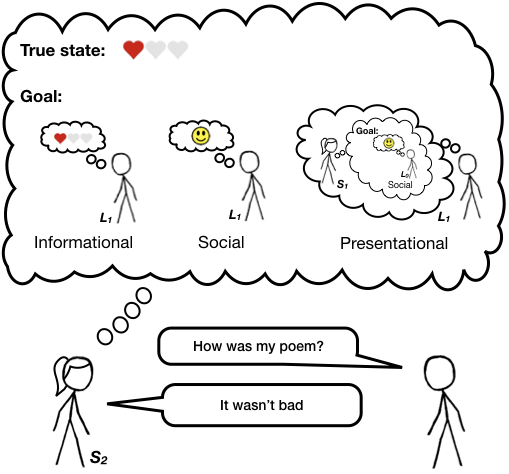
\includegraphics[width=0.6\textwidth]{fig/model} \centering \caption{Diagram of the model: The pragmatic speaker observes the true state and determines her goal between three utilities (informational, social, and presentational), and produces an utterance.}\label{fig:model}
\end{figure*}

RSA models are defined recursively such that speakers \(S\)  reason about
listeners  \(L\), and vice versa. We use convention in indexing and say a pragmatic listener \(L_1\) reasons about what intended meaning
and goals would have led a speaker \(S_1\) to produce a particular
utterance. Then \(S_1\) reasons about a \emph{literal listener}
\(L_0\), who is modeled as attending only to the literal meanings of words
(rather than their pragmatic implications), and hence grounds the
recursion.
The target of our current work is a model of a polite speaker \(S_2\)
who reasons about what to say to \(L_1\) by
considering informational, social, and self-presentational goals (Figure
\ref{fig:model}).

We evaluate our model on its ability to predict human utterance choices
in situations where polite language use is expected to varying degrees.
Imagine Bob gave a poem recital and asked Ann how good it was.
Ann (\(S_2\)) produces an utterance \(w\) based on the true state of the world \(s\) (i.e., the
rating, in her mind, truly deserved by Bob's poem) and a set of goal weights
\(\hat{\phi}\), that determines how much Ann prioritizes each of the three possible goals.
Ann's production decision is softmax, which interpolates between
maximizing and probability matching (via \(\lambda_{S_2}\); \cite{goodman2013}):

\begin{equation}
P_{S_2}(w | s, \hat{\phi}) \propto \exp(\lambda_{S_2} \cdot \mathop{\mathbb{E}}[U_{total}(w; s; \hat{\phi}; \phi_{S_1})]).
\end{equation}

We posit that a speaker's utility contains three distinct components: informational, social, and presentational. The
total utility $U_{total}$ of an utterance is thus the weighted combination of the three component utilities minus the utterance cost \(C(w)\):

\begin{equation}
\begin{split}
U_{total}(w; s; \hat{\phi}; \phi_{S_1}) = \phi_{inf} \cdot U_{inf}(w; s) + \phi_{soc} \cdot U_{soc}(w) + \\ \phi_{pres} \cdot U_{pres}(w; \phi_{S_1}) - C(w).
\end{split}
\end{equation}

%Aspects of the world with affective consequences for the listener (e.g., Bob and his pie) influence the social utilities in the model.
We define \emph{social utility} \(U_{soc}(w)\) as the expected subjective utility of the state \(V(s)\) implied to the
pragmatic listener by the utterance: \(U_{soc}(w) = \mathbb{E}_{P_{L_1}(s \mid w)}[V(s)]\).
The subjective utility function \(V(s)\) could vary by culture and context; we test our model when states are explicit ratings (e.g., on a 4-point scale) and we assume a positive linear value relationship between states and values \(V\) to model a listener's preference to be in a highly rated state (e.g., Bob would prefer to have written a poem deserving 4 points rather than 1 point).

At the same time, a speaker may desire to be epistemically helpful, modeled as standard \emph{informational utility} (\(U_{inf}\)).
The informational utility indexes the amount of information the listener (\(L_1\)) would still not know about the state of the world \(s\) after hearing the speaker's utterance \(w\) (i.e., surprisal; e.g., how likely is Bob to guess Ann's actual opinion of the poem): \(U_{inf}(w) = \ln(P_{L_1}(s | w))\).
Speakers who optimize for informational utility produce accurate and informative utterances while those who optimize for social utility produce utterances that make the listener feel good.

If a listener is uncertain how their particular speaker is weighing the competing goals to be honest vs. kind (i.e., informational vs. social), they might try to infer the weighting (e.g., ``was she just being nice?'').
But then a sophisticated speaker can produce utterances in order to appear \emph{as if} they had certain goals in mind (i.e., a self-presentational goal).
The extent to which the speaker \emph{appears} to the listener to have a particular goal in mind \(\phi_{S_1}\) (e.g., to be kind) is the utterance's \emph{presentational utility} (\(U_{pres}\)) and is the most novel component of our model.
The speaker gains presentational utility when her listener believes she
has particular goals, represented by a mixture weighting \(\phi_{S_1}\) between trying to be informative vs. kind.
Formally,

\begin{equation}
U_{pres}(w; \phi_{S_1}) = \ln(P_{L_1}(\phi_{S_1} \mid w)) = \ln \int_s P_{L_1}(s, \phi_{S_1} \mid w).
\end{equation}

The speaker conveys a particular weighting of informational
vs.~social goals (\(\phi_{S_1}\)) by considering the
beliefs of listener \(L_1\), who hears an utterance and jointly infers
the speaker's utilities and the true state of the world:

\begin{equation}
P_{L_1}(s, \phi_{S_1} | w) \propto P_{S_1}(w | s, \phi_{S_1}) \cdot P(s) \cdot P(\phi_{S_1}).
\end{equation}

The presentational utility is the highest-order term of the model, defined only for a speaker thinking about a listener who evaluates a speaker
(i.e., defined for \(S_2\), but not \(S_1\)).
Only the social and informational utilities are defined for the \(S_1\)) speaker (via reasoning about \(L_0\)); thus, \(S_1\)'s utility weightings can be represented by a single number, the mixture parameter \(\phi_{S_1}\).
Definitions for \(S_1\) and  \(L_0\) otherwise mirror those of  \(S_2\) and  \(L_1\) and can be found in the Supplementary Information.

Finally, more complex utterances incur a greater cost, \(C(w)\) --
capturing the general pressure towards economy in speech. In our work,
utterances with negation (e.g., \emph{not terrible}) are assumed to
be slightly costlier than their equivalents with no negation (and this cost differential is inferred
from data; see Supplementary Information).

Within our experimental domain, we assume there are four possible states
of the world corresponding to the value placed on a particular referent
(e.g., the poem the speaker is commenting on), represented in terms of numbers of hearts (Figure \ref{fig:model}):
\(S = {s_0,...,s_3}\). Since the rating scale is relatively abstract, we assume a uniform prior distribution
over possible states of the world. The set of utterances is
\{\emph{terrible}, \emph{bad}, \emph{good}, \emph{amazing}, \emph{not
terrible}, \emph{not bad}, \emph{not good}, and \emph{not amazing}\}. We
implemented this model using the probabilistic programming language
WebPPL \cite{dippl}.



%If Bob's pie was good, Ann's utilities align to produce a positive utterance.
%Saying \emph{{[}Your pie{]} was amazing} simultaneously is truthful, kind, and appears as both.
%If Bob's pie was poor, however, the speaker is in a bind: Ann could be kind and say \emph{It was great}, but at the cost of conveying the wrong information to Bob if he believes her to be truthful.
%If he does not, he might infer Ann is \emph{just being
%nice}, but is uninformative. Alternatively, she could say the truth
%(\emph{It was bad}), but then Bob would think Ann didn't care about
%him.
%What is a socially-aware speaker to do? Our quantitative model predicts that
%indirect speech -- like \emph{It wasn't bad} -- best navigates Ann's
%dilemma. Her statement is sufficiently open-ended to include the
%possibility that the pie was good, but her avoidance of the simpler and
%less costly \emph{It was good} provides both an inference available to Bob that the
%pie was mediocre and that Ann cares about his feelings by not saying the blunt truth.


\begin{figure}[!h]
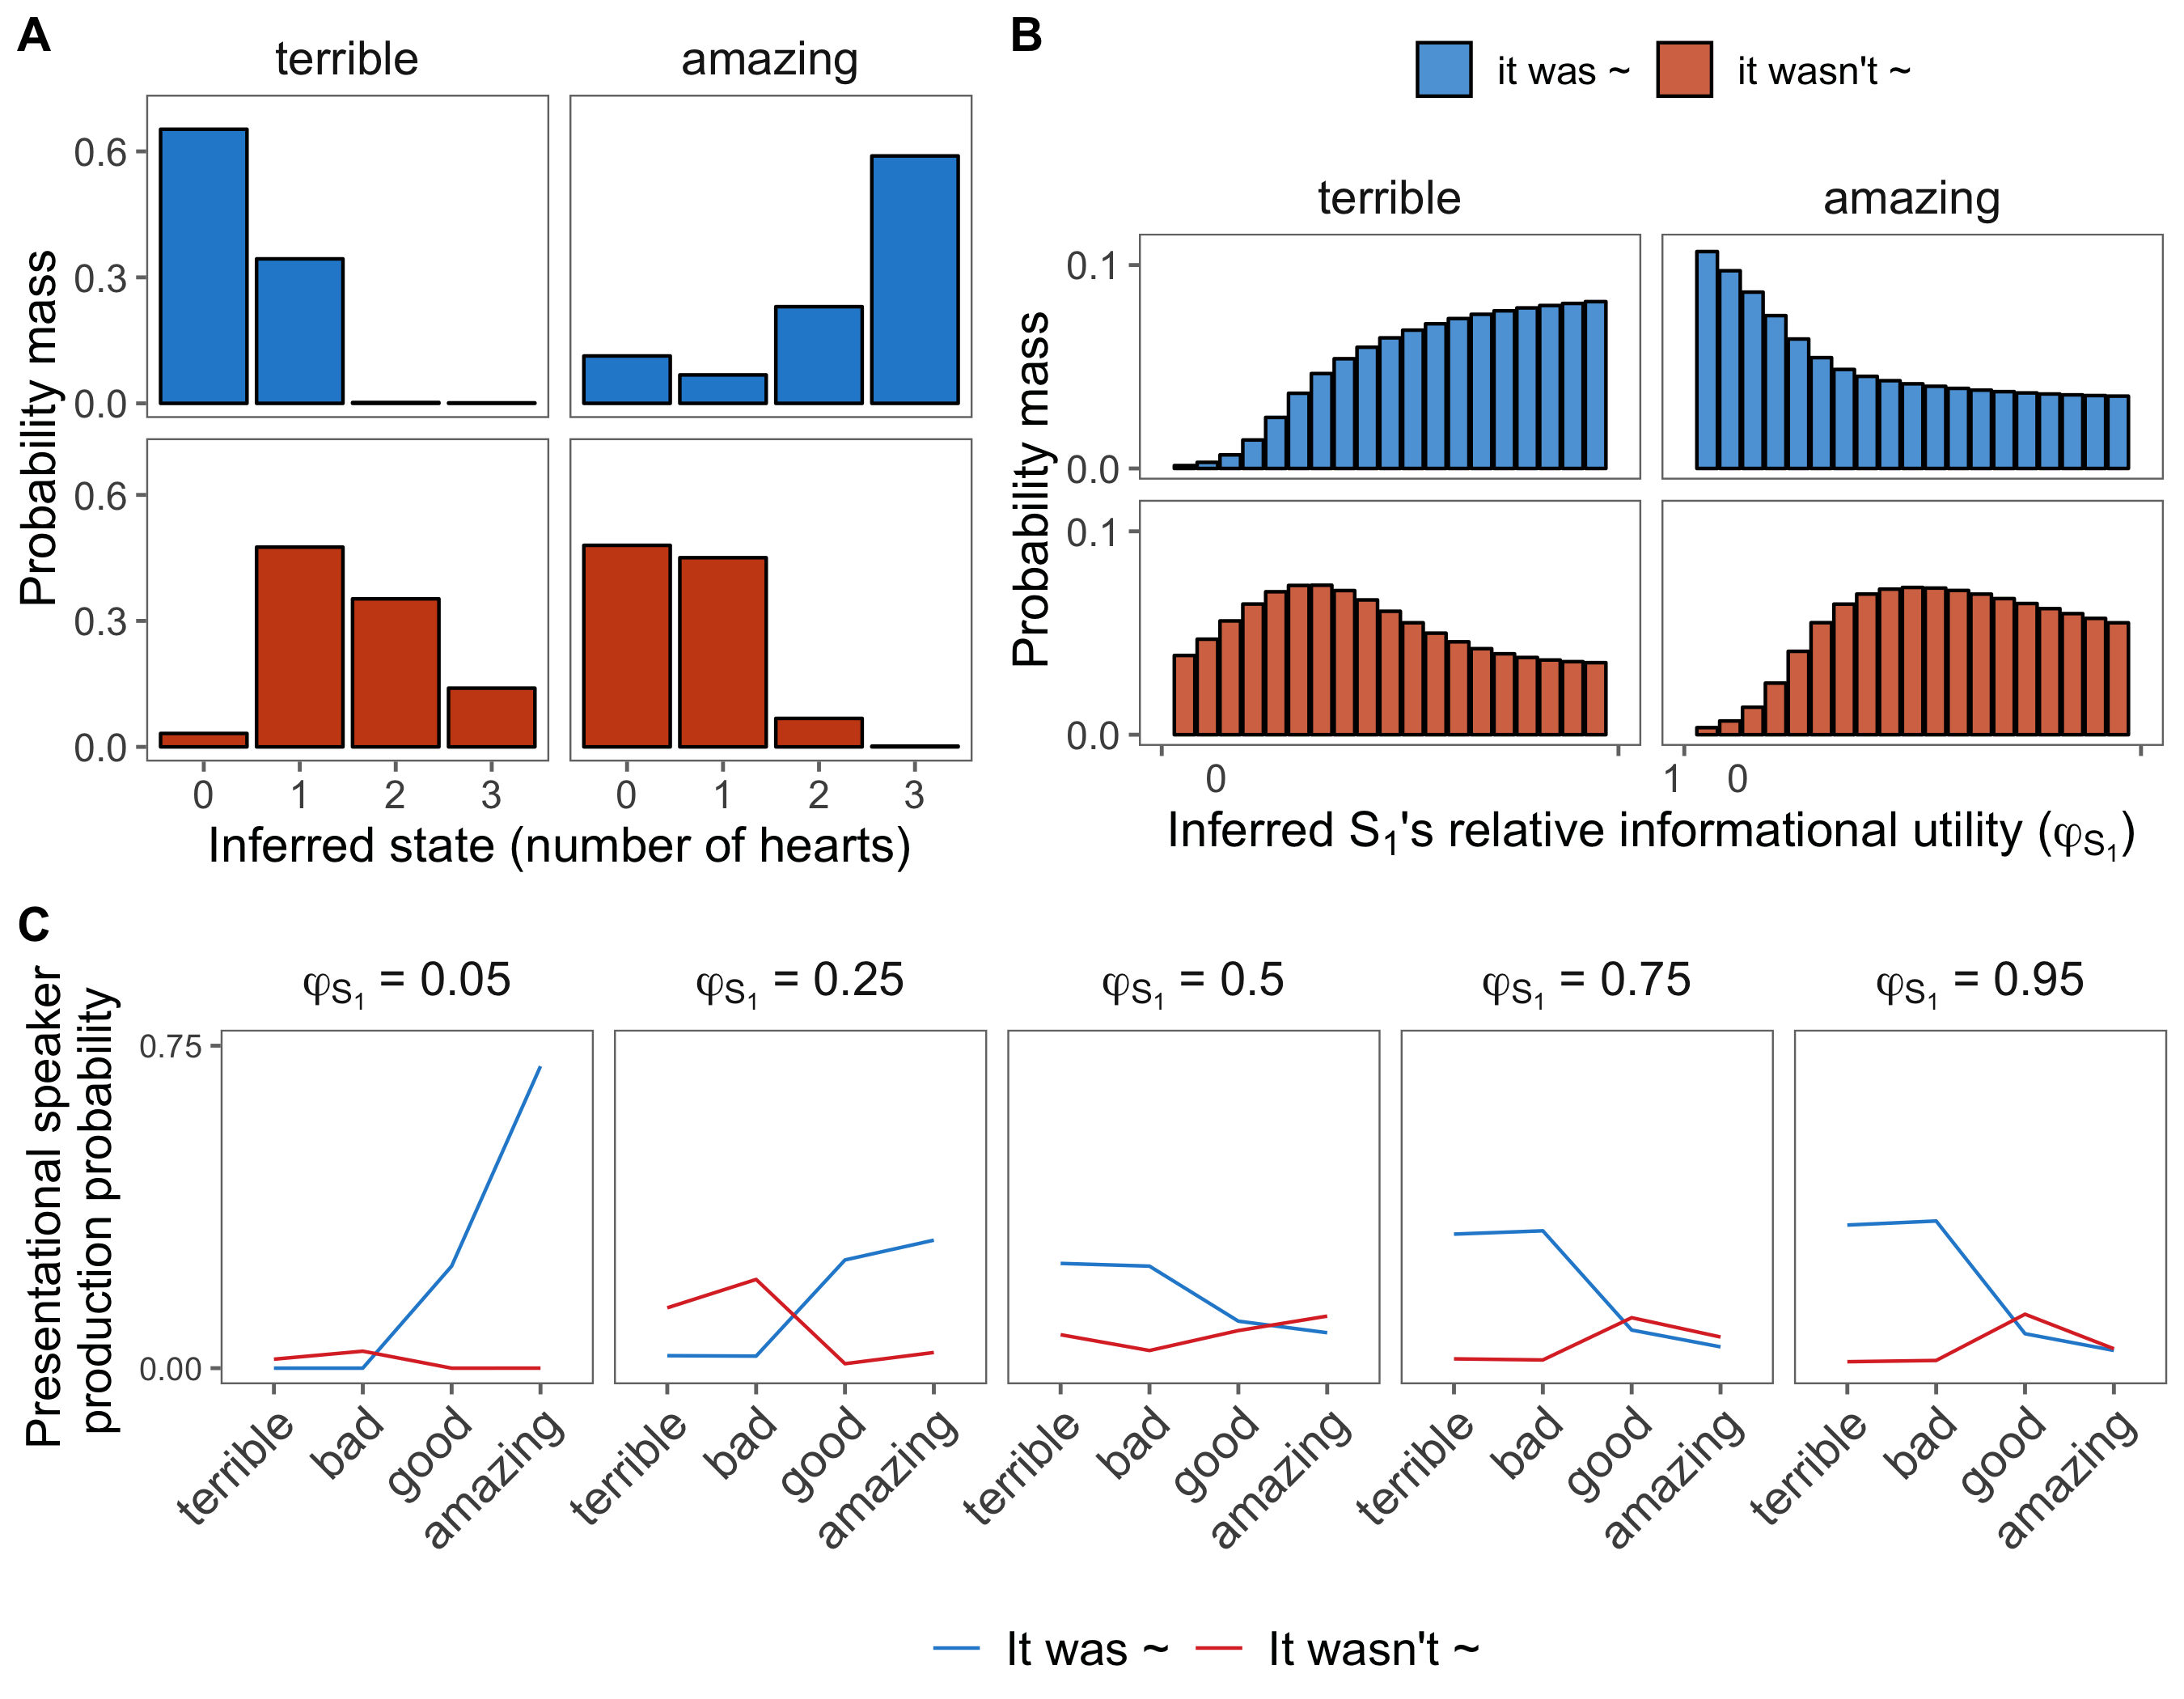
\includegraphics[width=\columnwidth]{fig/L1_inferences_wS2pres} \centering \caption{Model behavior. Listener inferences about the state (A) and the speaker's utility weighting (informational vs. social; B) as a function of the utterance heard (facets). C: Purely self-presentational speaker production behavior as a function of the kind of speaker they wish to present themselves as (facets; informational vs. social).}\label{fig:L1inferences}
\end{figure}


\section*{Results}

The pragmatic listener model \(L_1\) draws complex inferences about both the state of the world (Figure \ref{fig:L1inferences}A) and the speaker's goals (Figure \ref{fig:L1inferences}B).
Upon hearing \emph{{[}Your poem{]} was terrible} (Fig.~\ref{fig:L1inferences} top-left), the listener infers the poem is probably worthy of zero hearts and that the speaker has strong informational goals.
\emph{It was amazing} is more ambiguous (Fig.~\ref{fig:L1inferences} top-right): The poem could be worthy of three hearts but it's plausible the speaker had strong social goals and the poem was mediocre. 
Negation makes the meanings less precise and introduces more uncertainty into the inference about the state: A listener who hears \emph{It wasn't amazing} sees it as a relatively kind way of saying that the poem was quite bad (0 or 1 hearts), inferring a balance of social and informational goals for the speaker (Fig.~\ref{fig:L1inferences} bottom-right).
\emph{It wasn't terrible} is the most open-ended, leaving open the possibility that the poem was worthy of 0 hearts (i.e., \emph{it was terrible}) but conveying to the listener that the speaker cares about both informational and social goals, with a slight preference of towards being social (Fig.~\ref{fig:L1inferences} bottom-left). 

The self-presentational utility guides the speaker \(S_2\) to care about how she will be viewed in the eyes of the listener \(L_1\) (Figure \ref{fig:L1inferences}C).
If the speaker wants to present herself as someone who is socially-minded (e.g., informational mixture of 0.05), she should produce direct, positive utterances (e.g., \emph{amazing}).
The best way to appear honest (e.g., informational mixture of 0.95) is to say direct, negative utterances (e.g., \emph{terrible}).
The desire to appear as someone concerned with telling the truth while also caring about the listener's feelings (e.g., informational mixture of 0.25) leads the speaker to produce indirect utterances (e.g., \emph{not terrible}).
Such indirect speech acts are sufficiently open-ended to include the
possibility that the poem was good, but the avoidance of a more direct utterance (e.g., \emph{good}) provides the listener with a way to recover the true state (e.g., the poem was mediocre) by way of reasoning that the speaker cares about his feelings by not saying the blunt truth.

We made a direct, fully pre-registered test of our speaker production model and its performance in comparison to a range of alternative models, by instantiating our running example in an online experiment (\emph{N} = 202).
Participants read scenarios with information on the speaker's (Ann's,
in our example) feelings toward some performance or product (e.g., a poem
recital; \emph{true state}), on a scale from zero to three hearts (e.g.,
one out of three hearts). For example, one trial read: \emph{Imagine
that Bob gave a poem recital, but he didn't know how good it was. Bob
approached Ann, who knows a lot about poems, and asked} ``How was my poem?''


We manipulated the speaker's goals across trials: to be
\emph{informative} (\emph{give accurate and informative feedback});
to be \emph{kind} (\emph{make the listener feel good}); or to be
both informative and kind simultaneously. We hypothesized that
each of the three experimentally-induced goals would induce a different tradeoff between social and informational
utilities in our model as well as include a self-presentational component (i.e., some mixture of the three utilities; see Supplementary Information). In a single
trial, each scenario was followed by a question asking for the most
likely produced utterance by Ann. Participants selected one of eight possible
utterances, by choosing between \emph{It was} vs. \emph{It wasn't} and
then among \emph{terrible}, \emph{bad}, \emph{good}, and \emph{amazing.}

\begin{figure}[!h]
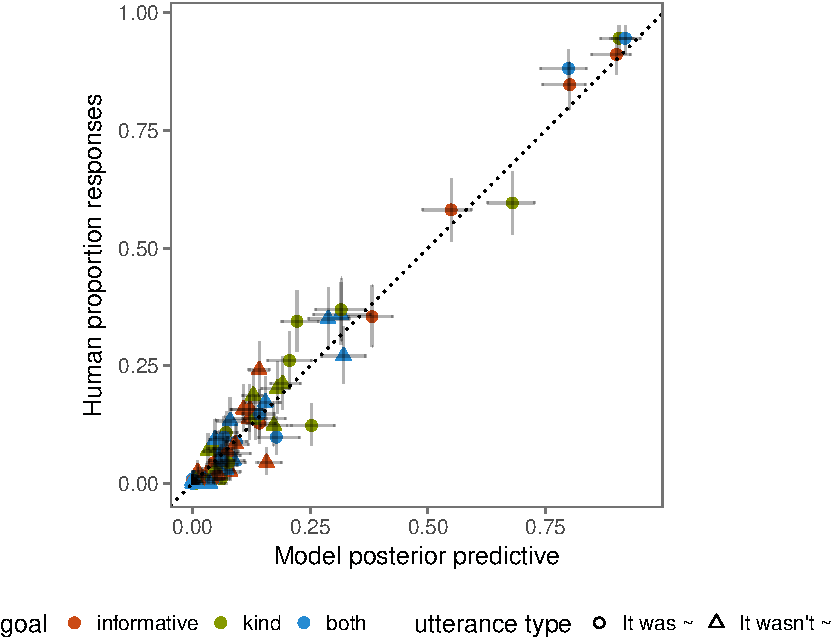
\includegraphics[width=0.5\textwidth]{fig/variance-1} \caption{Full distribution of human responses vs. model predictions. Error bars represent 95\% confidence intervals for the data (vertical) and 95\% highest density intervals for the model (horizontal).}\label{fig:variance}
\end{figure}

Our primary behavioral hypothesis was that speakers describing bad
states (e.g., Bob's poem deserved 0 hearts) with goals to be both
informative and kind would produce more indirect, negative utterances
(e.g., \emph{It wasn't terrible}). Such indirect speech acts both
save the listener's face and provide some information about the
true state, and thus, are the kind of thing that a socially-conscious speaker would say (Figure \ref{fig:L1inferences}).
This prediction was confirmed: a Bayesian mixed-effects
model predicts more negation as a function of true state and goal via
an interaction such that a speaker with both goals to be informative and
kind produced more negation in worse states compared to a speaker with
only the goal to be informative (\emph{M} = -1.33, {[}-1.69, -0.98{]})
and goal to be kind (\emph{M} = -0.50, {[}-0.92, -0.07{]}). Rather than
eschewing one of their goals to increase utility along a single
dimension, participants chose utterances that jointly satisfied their
conflicting goals by producing indirect, polite speech.

\begin{figure*}[!h]
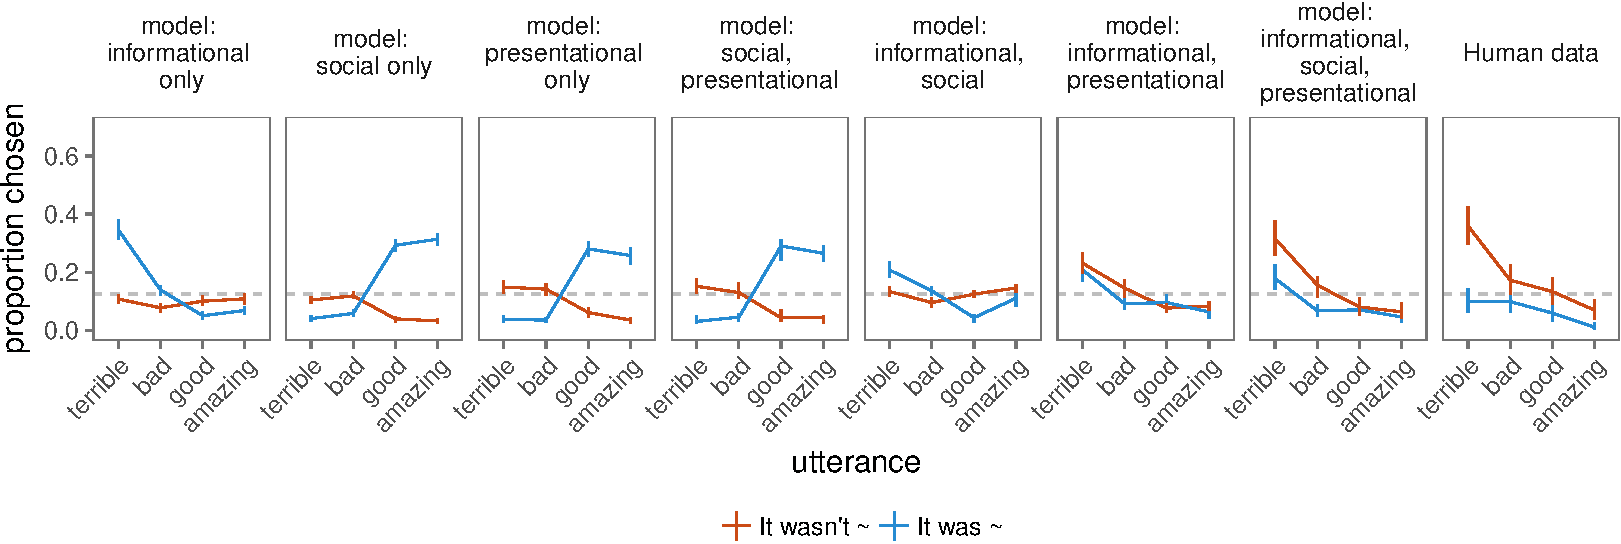
\includegraphics[width=\textwidth]{fig/comparison-1} \caption{Comparison of predictions for proportion of utterances chosen by pragmatic speaker from possible model variants (left) and human data (rightmost) for average proportion of negation produced among all utterances, given true state of 0 heart (on a scale of 0 to 3) and speaker with both goals to be informative and kind. Gray dotted line indicates chance level at 12.5\%.}\label{fig:comparison}
\end{figure*}

\begin{table}[tbp]
\begin{center}
\begin{threeparttable}
\caption{\label{tab:comparisonTable}Comparison of variance explained for each model variant and log Bayes Factors quantifying evidence in favor of alternative model in comparison.}
\begin{tabular}{lll}
\toprule
Model & \multicolumn{1}{c}{Variance
explained} & \multicolumn{1}{c}{log BF}\\
\midrule
model:
informational,
social,
presentational & 0.97 & --\\
model:
informational,
presentational & 0.96 & -11.14\\
model:
informational,
social & 0.92 & -25.06\\
model:
social,
presentational & 0.23 & -864\\
model:
presentational
only & 0.23 & -873.83\\
model:
social only & 0.22 & -885.52\\
model:
informational
only & 0.83 & -274.89\\
\bottomrule
\end{tabular}
\end{threeparttable}
\end{center}
\end{table}
The model parameters (softmax parameters and each goal condition's utility weights) can be inferred from the behavioral data using a Bayesian data analysis model (\cite{lee2014}; see Supplementary Information)
To approximate the literal meanings (i.e., the semantics) of the words as interpreted by the literal listener \(L_0\), we obtained literal meaning judgments from an independent group of participants
(\emph{N}=51).
The posterior predictions from the the three-utility polite speaker model (informational, social, presentational) showed a very strong fit to participants' actual utterance choices (\(r^2\)(96) = 0.97; Figure \ref{fig:variance}).
We compared these to six model variants containing
subsets of the three utilities in the full model.
Both the variance explained and the marginal likelihood of the observed data were the
highest for the full model (Table \ref{tab:comparisonTable}). Only the
full model captured participants' preference for negation when the speaker wanted to be informative and kind
about truly bad states, as hypothesized (Figure \ref{fig:comparison}).
In sum, the full collection of informational, social, and presentational were
required to fully explain participants' utterance choices.



\begin{table}[tbp]
%\resizebox{\columnwidth}{!}{
\begin{center}
\begin{threeparttable}
%\centering
\caption{\label{tab:phi}Inferred phi parameters from all model variants with more than one utility.}
%\begin{tabular}{llllll}
\begin{tabularx}{\columnwidth}{llllll}
\toprule
Model (utilities) & \multicolumn{1}{l}{goal} & \multicolumn{1}{c}{$\phi_{inf}$} & \multicolumn{1}{c}{$\phi_{soc}$} & \multicolumn{1}{c}{$\phi_{pres}$} & \multicolumn{1}{c}{$\phi_{S_1}$}\\
\midrule
inf, soc, pres & both & 0.36 & 0.11 & 0.54 & 0.36\\
inf, soc, pres & informative & 0.36 & 0.02 & 0.62 & 0.49\\
inf, soc, pres & social & 0.25 & 0.31 & 0.44 & 0.37\\
inf, pres & both & 0.64 & -- & 0.36 & 0.17\\
inf, pres & informative & 0.77 & -- & 0.23 & 0.33\\
inf, pres & social & 0.66 & -- & 0.34 & 0.04\\
inf, soc & both & 0.54 & 0.46 & -- & --\\
inf, soc & informative & 0.82 & 0.18 & -- & --\\
inf, soc & social & 0.39 & 0.61 & -- & --\\
soc, pres & both & -- & 0.38 & 0.62 & 0.55\\
soc, pres & informative & -- & 0.35 & 0.65 & 0.75\\
soc, pres & social & -- & 0.48 & 0.52 & 0.66\\
\bottomrule
\end{tabularx}
\end{threeparttable}
\end{center}
%}
\end{table}


The utility weights inferred for the three-utility model (Table \ref{tab:phi})
provide additional insight into how polite language use operates:
\emph{Being kind} requires equal weights on all three utilities,
indicating that Gricean informativity needs to be part of language use
even when it is explicitly not the goal.
\emph{Being informative} pushes
the weight on social utility close to zero, but the weight on
\emph{appearing kind} stays high, suggesting that speakers are expected
to manage their own face even when they are not considering others'.
\emph{Kind and informative} speakers emphasize informativity slightly
more than kindness. In all cases, however, the presentational utilities
have greatest weight, which may suggest that appearing honest and kind
is more important than actually being so! Overall then, our condition
manipulation altered the balance between these weights, but all
utilities played a role in all conditions.

\section*{Discussion}

Politeness is puzzling from an information-theoretic perspective.
Incorporating social motivations adds a level of explanation, but so far such intuitions and observations have resisted both formalization and precise testing.
% intuitions have been resistant to formalization or
We present a utility-theoretic model of language use that captures the interplay between competing
informational, social, and presentational goals, and provide preregistered
experimental evidence that confirmed its ability to capture human
judgments, unlike comparison models that used only a subset of the full
utility structure.

To precisely estimate choice behavior in the experiment,
it was required to abstract away
from natural interactions in a number of ways.
Human speakers have access
to a potentially infinite set of utterances to select from in order to manage the three-utility tradeoff (\emph{It's hard to write a good poem}, \emph{That
metaphor in the second stanza was so relatable!}). In theory,
each utterance will have strengths and weaknesses relative to the
speaker's goals, though computation in an unbounded model presents
technical challenges (perhaps paralleling the difficulty human speakers
feel in finding the right thing to say in a difficult situation; see \cite{goodman2016}).

For a socially-conscious speaker, managing listeners' inferences is a
fundamental task. Our work extends previous models of language beyond
standard informational utilities to address social and
self-presentational concerns. Further, our model builds upon the theory of politeness as face
management \cite{brown1987} and takes a step towards
understanding the complex set of social concerns involved in face management.
% This work breaks through to exploring how informational cooperativity interacts
% with other social goals, and
Our approach can provide insight into a wide range of social behaviors beyond speech by considering utility-driven inferences in a
social context \cite{baker2017rational, hamlin2013mentalistic} where agents need to take
into account concerns about both self and others.

Previous game-theoretic analyses of politeness have either required some social cost to an utterance (e.g., by reducing one's social status or incurring social debt to one's conversational partner; \cite{vanRooy2003}) or a separately-motivated notion of plausible deniability \cite{pinker2008}.
The kind of utterance cost for the first type of account would necessarily involve higher-order reasoning about other agents, and may be able to be defined in terms of the more basic social and self-presentational goals we formalize here.
A separate notion of plausible deniability may not be needed to explain most politeness behavior, either.
Maintaining plausible deniability is in one's own self-interest (e.g., due to controversial viewpoints or covert deception) and goes against the interests of the addressee; some amount of utility dis-alignment is presumed by these accounts. Politeness behavior appears present even in the absence of obvious conflict, however: in fact, you might be even more motivated to be polite to someone whose utilities are more aligned with yours (e.g., a friend). In our work here, we show that such behaviors can in fact arise from purely cooperative goals \cite{brown1987}, though our account is not inconsistent with the invocation of plausible deniability accounts in cases of conflict.

%balance cooperation and conflict between interlocutors (e.g., in deception), which characterized human politeness intuitions
%Here we show indirectness arising from purely cooperative goals, which address different aspects of a general utility structure.

% to indirect speech but here we show indirectness arising from (Pinker, Nowak, and Lee, 2008)
%In such a model, utterance cost requires a component derived from the social world (e.g., an utterance may be costly by reducing one's social status or incurring social debt to one's conversational partner; , but it's not clear how cost should be determined nor how it generalizes to other politeness behavior (e.g., evaluative statements like those made in our experiment).
%Our model derives its predictions by construing the speaker utility as a collection of possible goals (here, epistemic,
%social, and presentational goals); utterance cost may strengthen the inferences, but it is not a fundamental necessity.
%The speech-acts themselves are not costly.
%
%Pinker, Nowak, and Lee (2008) model game-theoretic communication as involving a mixture of cooperation
%\emph{and} conflict: indirect speech allows for plausible deniability, which is in one's own self-interest but goes against the interest of the addressee.
%Our work sees polite speech as fundamentally cooperative, building on classic theories of pragmatic language use (Brown \& Levinson, 1987;
%Grice, 1975).
%A separate notion of plausible deniability may not be needed:
%Indirect speech in our case study comes from both a goal to be
%helpful and a desire to look good.



%Van Rooy (2003)'s analysis relies on the notion that polite language is costly (in a social way
%e.g., by reducing one's social status or incurring social debt to one's
%conversational partner) but it's not clear how the polite behaviors
%explored in our experiments (not polite requests) would incur any cost
%to speaker or listener.
%
%pragmatics has offered
%
%. Van Rooy (2003) argues the
%purpose of polite language is to align the preferences of interlocutors.
%Our notion of social utility \(U_{soc}\) and presentational utility
%\(U_{pres}\) is similar in that they motivate speakers to signal worlds
%that make the listener feel good.

Utility weights and value functions in our model could provide a framework for a quantitative understanding of systematic
cross-cultural differences in what counts as polite. Cross-cultural differences in politeness could be a product of different weightings within the same
utility structure. Alternatively, culture could affect
the value function \(V\) that maps states of the world onto subjective
values for the listener (e.g., the mapping from states to utilities may
be nonlinear and involve reasoning about the future).
Our formal modeling approach with systematic behavior measurements provides an avenue towards understanding the vast range of politeness practices found across languages.

We flirt, insult, boast, and empathize by balancing informative transmissions with goals to affect others' feelings or
present particular views of ourselves.
Politeness is only one of the ways that language use deviates from purely
informational transmission.
Our work shows how social and
self-presentational motives are integrated with informational concerns more
generally, opening up the possibility for a broader theory of social
language.
Finally, a formal account of politeness moves us closer to
courteous computation -- to machines that can talk with tact.

\matmethods{

\subsection*{Literal semantic task}\label{literal-semantic-task}

We probed judgments of literal meanings of the target words assumed by
our model and used in our main experiment. 51 participants with IP
addresses in the United States were recruited on Amazon's Mechanical
Turk. We used thirteen different context items in which a speaker
evaluated a performance of some kind. For example, in one of the
contexts, Ann saw a presentation, and Ann's feelings toward the
presentation (true state) were shown on a scale from zero to three
hearts (e.g., two out of three hearts filled in red color; see
Figure~\ref{fig:screenshot} for an example of the heart scale). The
question of interest was \emph{Do you think Ann thought the
presentation was / wasn't X?} and participants responded by choosing
either \emph{no} or \emph{yes.} The target could be one of four
possible words: \emph{terrible}, \emph{bad}, \emph{good}, and
\emph{amazing}, giving rise to eight different possible utterances (with
negation or no negation). Each participant read 32 scenarios, depicting
every possible combination of states and utterances. The order of
context items was randomized, and there were a maximum of four repeats
of each context item per participant. For this and the speaker
production experiment, we analyzed the data by collapsing across context
items. For each utterance-state pair, we computed the posterior
distribution over the semantic weight (i.e., how consistent X utterance
is with Y state) assuming a uniform prior over the weight (i.e., a
standard Beta-Binomial model). Meanings of the words as judged by
participants were as one would expect (Figure ~\ref{fig:litsem}).

\begin{figure}[!h]
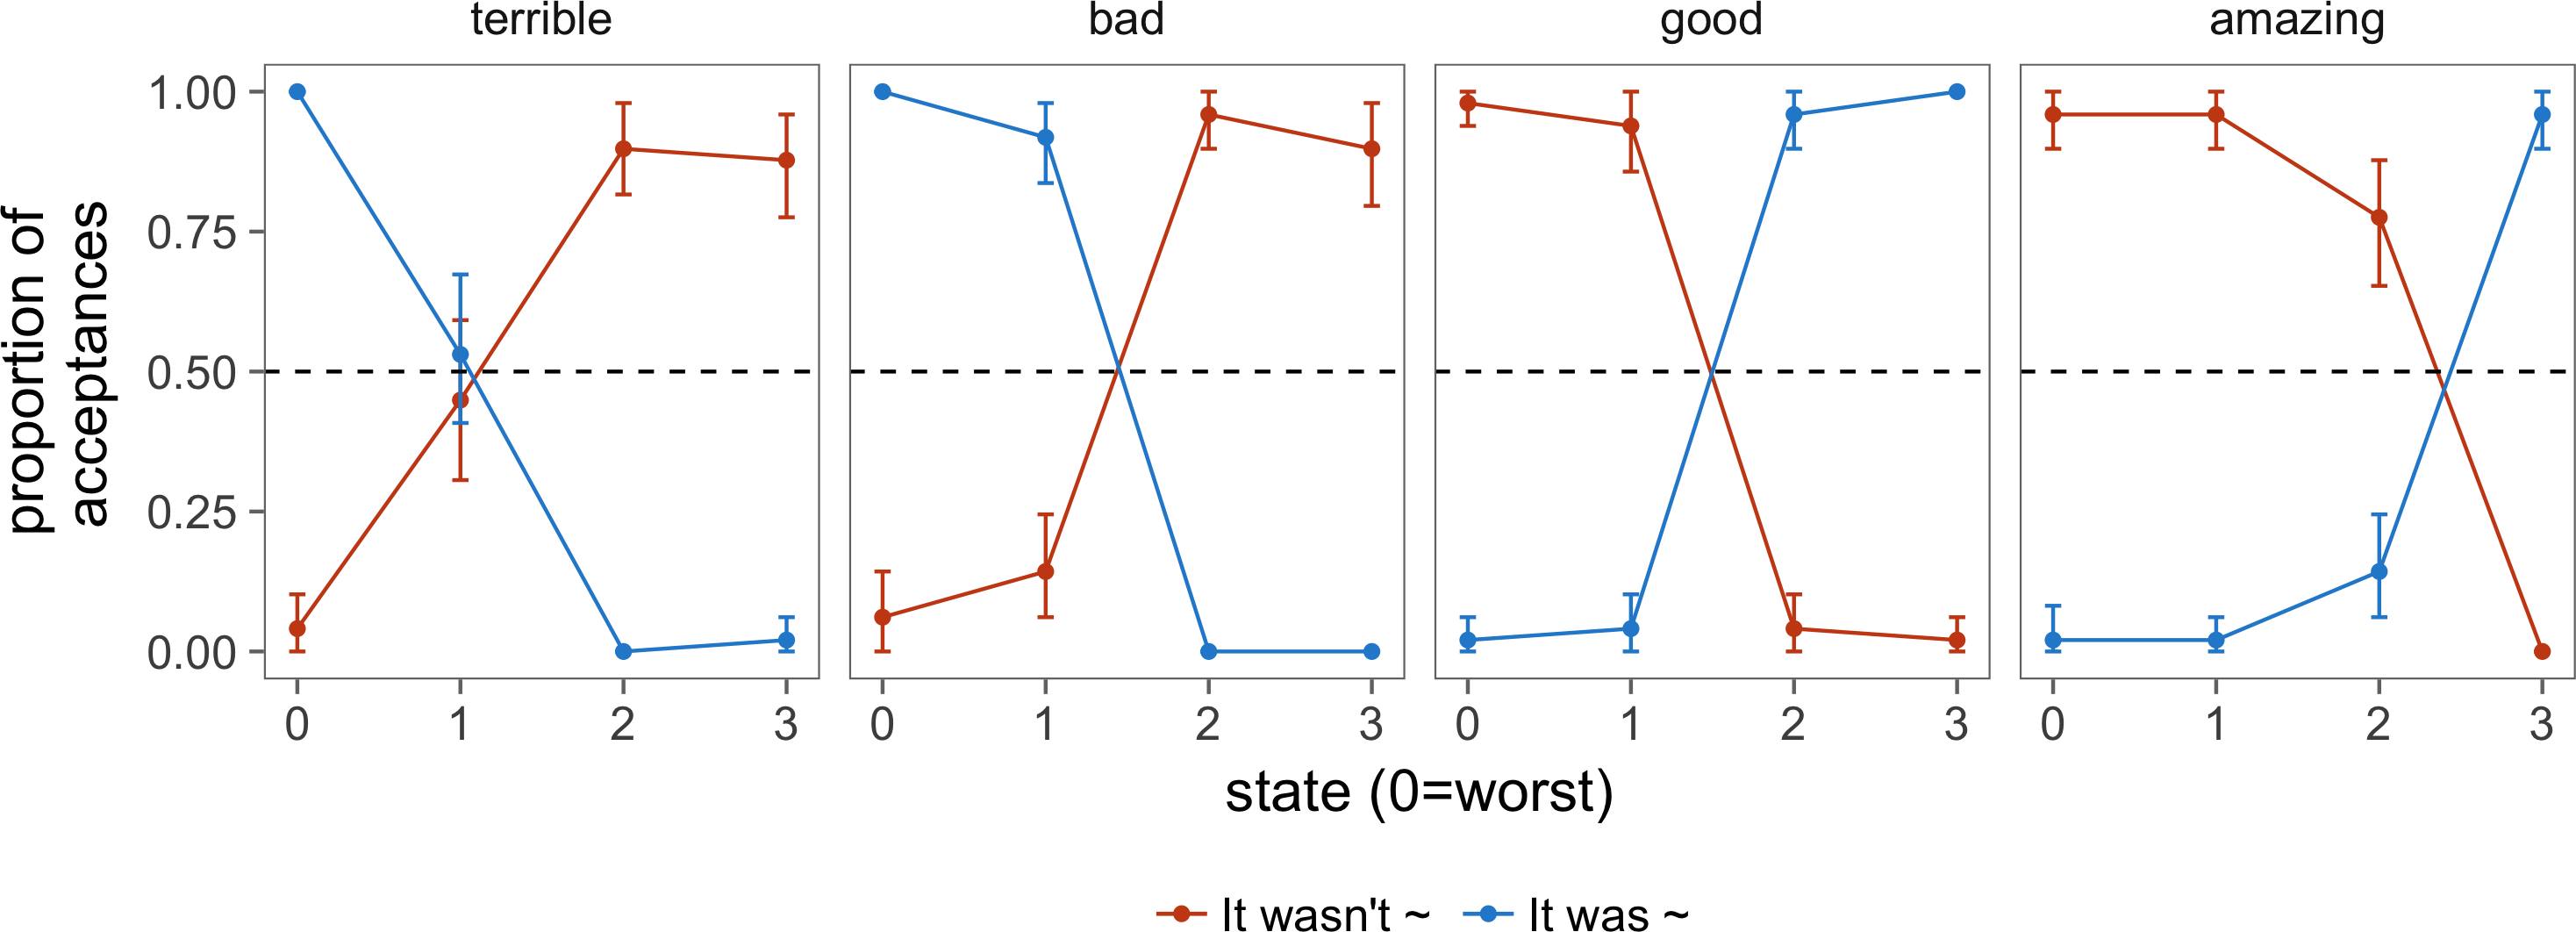
\includegraphics[width=\columnwidth]{fig/litsem-1}
\centering \caption{Semantic measurement results. Proportion of acceptances of utterance types (shown in different colors) combined with target words (shown in different facets) given the true state represented on a scale of hearts. Error bars represent 95\% confidence intervals.}\label{fig:litsem}
\end{figure}

\subsection*{Speaker production task}\label{speaker-production-task}

\begin{figure}[!h]
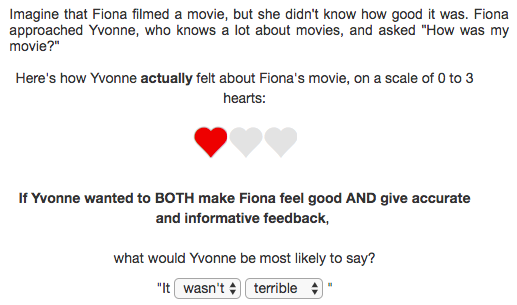
\includegraphics[width=\columnwidth]{fig/screenshot}
\caption{Example of a trial in the speaker production task.}\label{fig:screenshot}
\end{figure}

202 participants with IP addresses in the United States were recruited
on Amazon's Mechanical Turk. As in the literal semantic task above, we
used scenarios in which a person (e.g., Bob) gave some performance and
asked for another person (e.g., Ann)'s opinion on the performance
(Figure ~\ref{fig:screenshot}). Additionally, we provided information on
the speaker Ann's goal -- to make Bob feel good, or to give as accurate
and informative feedback as possible, or both -- and the true state --
how Ann actually felt about Bob's performance (e.g., two out of three
hearts, on a scale from zero to three hearts;
Figure~\ref{fig:screenshot}). Each participant read twelve scenarios,
depicting every possible combination of the three goals and four states.
The order of context items was randomized, and there were a maximum of
two repeats of each context item per participant. Each scenario was
followed by a question that read, \emph{If Ann wanted to make Bob
feel good but not necessarily give informative feedback (or to give
accurate and informative feedback but not necessarily make Bob feel
good, or BOTH make Bob feel good AND give accurate and informative
feedback), what would Ann be most likely to say?} Participants indicated
their answer by choosing one of the options on the two dropdown menus,
side-by-side, one for choosing between \emph{It was} vs. \emph{It
wasn't} and the other for choosing among \emph{terrible}, \emph{bad},
\emph{good}, and \emph{amazing.}

\subsection*{Data availability}\label{data-availability}

Our model, preregistration of hypotheses, procedure, data, and analyses
are available at \url{https://github.com/ejyoon/polite_speaker}.

}

\showmatmethods{} % Display the Materials and Methods section


\acknow{
This work was supported by NSERC PGS Doctoral scholarship
PGSD3-454094-2014 to EJY, NSF Graduate Research Fellowship DGE-114747 to
MHT, ONR grant N00014-13-1-0788 to NDG, and NSF grant BCS 1456077 to
MCF.
}

\showacknow{} % Display the acknowledgments section

% Bibliography
\bibliography{politeness}

\end{document}
